\chapter{随机动力学：从 Itô 公式到反向 SDE 与概率流}
\label{th:dynamics}

\section{布朗运动、二次变差与随机积分}

标准布朗运动 $W_t$ 从0开始，具有连续轨迹和独立高斯增量，
$W_{t+h}-W_t\sim\mathcal N(0,hI)$。增量尺度是 $\sqrt h$，不是 $h$。
沿越来越细的分割，平方增量之和趋向时间长度，即二次变差 $[W]_t=t$。
因此在微分运算中 $\mathrm dW\,\mathrm dW^\top=I\mathrm dt$，
而 $\mathrm dt\,\mathrm dW$ 与 $\mathrm dt^2$ 是更高阶量。

Itô 积分用区间左端、只依赖已知历史的被积函数定义。
若 $H_t$ 适应于过滤且平方可积，
\[
\E\int_0^T H_t\,\mathrm dW_t=0,\qquad
\E\left\|\int_0^T H_t\,\mathrm dW_t\right\|^2
=\E\int_0^T\|H_t\|_F^2\,\mathrm dt.
\]
这是 Itô 等距。随机积分不等于把一条不可导的布朗轨迹当普通函数积分。
Stratonovich 积分有另一种取点约定，转换会改变漂移；本文全部使用 Itô 约定。

\section{Itô 公式与生成算子}

考虑 $d$ 维过程
\[
\mathrm dX_t=f(X_t,t)\,\mathrm dt+G(X_t,t)\,\mathrm dW_t,
\qquad A=GG^\top.
\]
对 $C^{1,2}$ 测试函数 $\varphi(t,x)$，二阶 Taylor 展开保留噪声平方项，得到
\begin{equation}\label{th:ito}
\mathrm d\varphi=
\left(\partial_t\varphi+f\cdot\nabla\varphi
 +\tfrac12\tr(A\nabla^2\varphi)\right)\mathrm dt
 +(\nabla\varphi)^\top G\,\mathrm dW_t.
\end{equation}
生成算子作用于状态函数：$\mathcal L_t\varphi=f\cdot\nabla\varphi+
\tfrac12\tr(A\nabla^2\varphi)$。
适当边界与正则条件下，取期望再分部积分可得
\begin{equation}\label{th:fpe-general}
\partial_t p=-\sum_i\partial_i(f_ip)
 +\tfrac12\sum_{i,j}\partial_i\partial_j(A_{ij}p).
\end{equation}
左侧是时间导数；只有讨论稳定密度时才令它为0。
当 $G=g(t)I$ 时，扩散项化为 $\tfrac12g(t)^2\Delta p$。

\section{OU 过程：一个能核对全部符号的例子}

对 $\kappa>0$，令 $\mathrm dX_t=-\kappa X_t\mathrm dt+\sigma\mathrm dW_t$，
$X_0=x_0$。乘积分因子 $e^{\kappa t}$ 后积分：
\[
X_t=e^{-\kappa t}x_0+\sigma\int_0^t e^{-\kappa(t-r)}\mathrm dW_r.
\]
于是
\begin{equation}\label{th:ou}
X_t\mid x_0\sim\mathcal N\left(e^{-\kappa t}x_0,
 \frac{\sigma^2}{2\kappa}(1-e^{-2\kappa t})I\right).
\end{equation}
对应前向方程为 $\partial_t p=\kappa\nabla\cdot(xp)+
\tfrac12\sigma^2\Delta p$；稳定分布为 $\mathcal N(0,\sigma^2/(2\kappa)I)$。
均值应乘 $e^{-\kappa t}$，方差应非负且含 $1/2$ 因子。
这个例子可检查原稿中漂移符号、转移密度和稳定方差的错误。

\section{反向时间的两种写法}

先限制为 $G=g(t)I$，令真实分数为 $s_t=\nabla\log p_t$。
在密度平滑、正且满足时间反演条件时，反向过程可写为
\begin{equation}\label{th:reverse-negative-time}
\mathrm dX_t=[f(X_t,t)-g(t)^2s_t(X_t)]\mathrm dt
 +g(t)\mathrm d\bar W_t,\qquad t:T\downarrow0.
\end{equation}
这里时间增量为负，布朗增量协方差为 $|\mathrm dt|I$。
如用反向时钟 $r=T-t$，令 $Y_r=X_{T-r}$，则
\begin{equation}\label{th:reverse-positive-time}
\mathrm dY_r=[-f(Y_r,T-r)+g(T-r)^2s_{T-r}(Y_r)]\mathrm dr
 +g(T-r)\mathrm dB_r.
\end{equation}
后一式使用正步长，更便于检查代码的符号。
两式不能只改变时间变量而不改变漂移符号。

状态相关 $A(x,t)$ 时，还出现矩阵散度项。
在正向时刻、负步长写法中，反向漂移为
$f-\nabla\cdot A-A\nabla\log p$，其中
$(\nabla\cdot A)_i=\sum_j\partial_jA_{ij}$。
常用的 $f-g^2s$ 是时间依赖标量扩散的特例。

\section{从 Fokker--Planck 推出概率流 ODE}

利用 $\Delta p=\nabla\cdot(p\nabla\log p)$，
标量扩散的前向方程可以改写成
\[
\partial_t p=-\nabla\cdot\left[p\left(f-\tfrac12g^2s_t\right)\right].
\]
因此确定性速度
\begin{equation}\label{th:pf-ode}
u_t(x)=f(x,t)-\tfrac12g(t)^2s_t(x)
\end{equation}
的 ODE 与该 SDE 满足同一边缘演化方程。
反向积分 ODE 时仍使用负 $\mathrm dt$，无需再把速度取负。
反向 SDE 的系数是 $g^2$，概率流 ODE 是 $g^2/2$。

更一般地，已知速度 $u$ 与密度 $p_t$ 后，任意时间函数 $\eta(t)\geq0$
定义的正向 SDE
\[
\mathrm dX_t=\left[u_t+\tfrac12\eta(t)^2s_t\right]\mathrm dt+
\eta(t)\mathrm dW_t
\]
也满足相同的边缘连续性方程。这个构造不保证相同轨迹或耦合；
精确分数和完全匹配的边界分布是理论前提。

\begin{figure}[htbp]
\centering
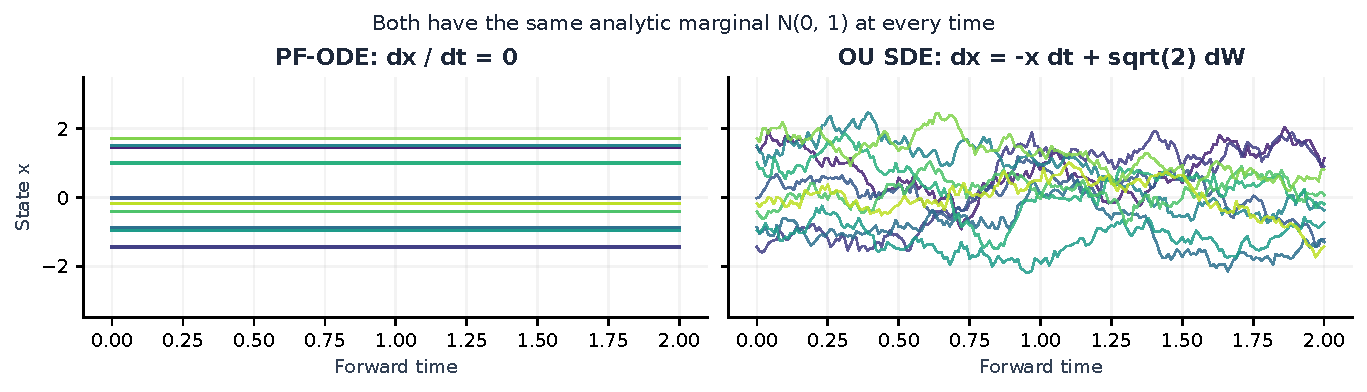
\includegraphics[width=\linewidth]{assets/theory/same-marginals.pdf}
\caption{同边缘不等于同轨迹：稳定 OU 过程取 $f=-x,g=\sqrt2,s=-x$，
其概率流速度为0。两者各时刻都服从标准高斯；左为静止的 ODE 轨迹，
右为用精确 OU 转移抽取的教学随机轨迹，未据有限样本估计分布等价。}
\end{figure}

\section{沿 ODE 计算似然}

对确定性速度 $u_\theta$，把观测 $x_0$ 正向积分到 $x_T$，
由式\eqref{th:cnf-density} 得
\begin{equation}\label{th:likelihood}
\log p_\theta(x_0)=\log p_T(x_T)+\int_0^T
 \nabla\cdot u_\theta(x_t,t)\,\mathrm dt.
\end{equation}
高维散度可用 Hutchinson 估计：若 $\E[ee^\top]=I$，
$\tr J=\E[e^\top Je]$。一次 Jacobian--vector 或向量--Jacobian 乘积
可避免显式形成 $d\times d$ Jacobian，但随机迹估计与数值积分各有误差。
“可计算模型似然”与“最大似然训练已完成”不是同一个命题。

\Needspace{17\baselineskip}
\section{Girsanov 为何把漂移误差变成路径 KL}

两个过程使用相同、非退化的扩散 $g(t)I$，漂移差为 $\delta_t$。
在绝对连续性与 Novikov 等可积条件成立时，路径相对熵包含
$\tfrac12\E\int\|\delta_t/g(t)\|^2\mathrm dt$。
对两条反向 SDE，若差只来自分数，$\delta_t=g(t)^2(s_\theta-s_t)$，
在精确反向路径作为期望分布时，得到
\begin{equation}\label{th:path-kl}
\KL(P\Vert P_\theta)=\KL(p_T\Vert\pi_T)
 +\tfrac12\int_0^T g(t)^2\E_{p_t}\|s_\theta-s_t\|^2\mathrm dt.
\end{equation}
$\pi_T$ 是实际使用的生成先验。路径投影的数据处理不等式进一步给出端点 KL 上界。
这条式子要求定义相同扩散与相容路径空间；不能把它直接当确定性 ODE 路径 KL，
也没有包含有限步采样的离散化误差。接近 $g=0$ 或奇异端点时需截断或单独分析。

\begin{theorytakeaway}
概率流的二分之一系数来自把扩散通量写成确定性速度。
时间反演、边缘等价、路径误差和数值误差各有条件；先固定时钟，再推公式。
\end{theorytakeaway}
\threading{主参考第4章、附录A--C及 Score SDE 原论文\cite{theorybook,sde}。
正文展示生成建模需要的随机分析核心，不把形式微分当作无条件成立的严格定理。}
